\documentclass[12pt,letterpaper]{article}

%{{{ Package configuration
%%%%%%%%%%%%%%%%%%%%%%%%%%%%%%%%%%%%%%%%%%%%%%%%%%%%%%%%%%%%%%%%%%%%%%%%%%%%%%%%

% Page margin
\usepackage[margin=1in]{geometry}

% Support for bold small cap font
\usepackage[tuenc]{fontspec}
\setmainfont[
    Path=./fonts/,
    Extension=.otf,
    BoldFont=cmu-serif-bold,
    BoldItalicFont=cmu-serif-bold-italic,
    ItalicFont=cmu-serif-italic,
]{cmu-serif}

% Better typesetting quality
\usepackage{microtype}

% Make letter spacing work for both XeLaTeX and LuaLaTeX
\usepackage{ifluatex}
\ifluatex
    \newcommand{\LSSTYLE}{\lsstyle}
\else
    \newcommand{\LSSTYLE}{\addfontfeatures{LetterSpace=12}}
\fi

% Math
\usepackage{amsmath}
\renewcommand{\vec}[1]{\mathbf{#1}}                   % Bold as vector
\newcommand{\spin}[1]{#1}                             % spinor doing nothing
\newcommand{\Lden}[1]{\ensuremath{\mathcal{L}_{#1}}}  % Lagrangian density

% SI units
\usepackage{siunitx}

% Figure
\usepackage{float,graphicx}

% Feynman slash notation
\usepackage{centernot}
\newcommand{\fsl}[1]{\ensuremath{\centernot{#1}}}

% Redefine section, subsection styles
\usepackage[compact,center,explicit]{titlesec}
\usepackage{textcase}
\titleformat{\section}{\LSSTYLE\normalsize\scshape\filcenter}
    {\thesection}{1em}{\MakeTextUppercase{#1}}
\titleformat{\subsection}{\small\bfseries\filcenter}
    {\thesubsection}{1em}{#1}

% PRL-style horizontal rule
\usepackage{amssymb}
\newcommand{\PRLrule}{
    \bigskip
    \noindent\makebox[\linewidth]{
        \resizebox{0.3333\linewidth}{1pt}{$\blacklozenge$}
    }
    \bigskip
}

% Bold math in section title
\makeatletter
\g@addto@macro\bfseries{\boldmath}
\makeatother

% Set up author affiliation
\usepackage[affil-it]{authblk}

% Set up link, with (hopefully) math symbol support
\usepackage[pdfencoding=auto,psdextra]{hyperref}
\hypersetup{colorlinks,breaklinks,citecolor=blue}
\usepackage{cleveref}

% Set up bibliography
\usepackage[
    %style=phys,
    giveninits=true,
    %backref=true,
    natbib=true,
    backend=biber,
    doi=true,
    % Sort by the order of citation
    sorting=none,
    % This options ensures that no automatic et al. is generated
    %maxbibnames=99,
    % This option must be enabled with 'babel' package
    useprefix=false
]{biblatex}
\addbibresource{umd_phd_candidacy_paper.bib}

%}}}

%{{{ User settings
%%%%%%%%%%%%%%%%%%%%%%%%%%%%%%%%%%%%%%%%%%%%%%%%%%%%%%%%%%%%%%%%%%%%%%%%%%%%%%%%

% User-defined variables
\def\BaBar/{\textsc{BaBar}}
\def\Y4S/{\ensuremath{\Upsilon(\text{4S})}}
\def\RD/{\ensuremath{\mathcal{R}(D)}}
\def\RDst/{\ensuremath{\mathcal{R}(D^{*})}}
\def\RDDst/{\ensuremath{\mathcal{R}(D^{(*)})}}

% Title info
\title{Review on testing lepton flavor universality in semileptonic channels}
\author{Yipeng Sun}
\affil{Department of Physics, University of Maryland}
\date{\today}

%}}}

\begin{document}
\maketitle

\begin{abstract}
    What is LFUV? (FU physics, FUV physics)
    Why semileptonic decays (good thing about form factor)?
    A historical review, starting from 2012 BaBar;
    Talk about Phoebe's run 1 analyses.
    Talk about what we are doing.
    Talk about expected improvements and drawbacks of our upcoming analysis compared
    to run 1.
\end{abstract}

\section{Introduction}
The Standard Model (SM) has been very successful in describing the interactions
between elementary particles such as quarks and leptons.
The theory has been tested experimentally to a very high precision.
However, there are phenomena that cannot be explained by the SM, such as
the observed matter-antimatter asymmetry in the universe, hinting that there might be New Physics (NP) beyond the SM.
One way to search for NP is to measure the decay rates of certain processes
very precisely;
rates that differ from the SM predictions may provide evidence for NP.

Through experimental discovery, it has been established that leptons have three
flavors:
Charged leptons, namely electron $e$, muon $\mu$, and tau $\tau$;
their corresponding charge-neutral neutrinos: $\nu_e$, $\nu_\mu$ and $\nu_\tau$.
SM assumes that all three flavors of leptons participate in all
interactions with the same strength, except for the Higgs mechanism through which
they acquire their mass.
This is known as lepton flavor universality (LFU).

LFU has been tested in many precision measurements, such as the decay rate
of $K^- \rightarrow e^- \nu_e$ versus $K^- \rightarrow \mu^- \nu_\mu$\footnote{
    Unless specified, charge conjugation is assumed throughout the paper.
}.
So far, no definite violation of LFU has been detected.

In this paper, we focus on the semileptonic decays of $B$ mesons, such as
$B^- \rightarrow D^{(*)} l^- \overline{\nu}_l$:
Currently, the world average of the combined decay rate ratio $\RDDst/$,
defined as\footnote{
    $\mathcal{B}$ denotes branching fraction.
}:
\begin{equation}
    \RDDst/ \equiv \frac{
        \mathcal{B}\left(
            B^{0,-} \rightarrow D^{+,0(*)} \tau^- \overline{\nu}_\tau
        \right)
    }{
        \mathcal{B}\left(
            B^{0,-} \rightarrow D^{+,0(*)} \mu^- \overline{\nu}_\mu
        \right)
    }
\end{equation}
has a $3.08\sigma$ deviation from the SM prediction \cite{HFLAV:2019}, pointing
to a possible lepton flavor universality violation (LFUV);
many collaborations are working on more precise measurements to provide a
definite answer.

In this paper, we begin with a theoretical review on
why SM manifests LFU;
extensions to SM, such as 2-Higgs doublet model (2HDM), to permit LFUV;
and advantages of using semileptonic channels for this type of measurements.
We then review and compare colliders and detectors, such as \BaBar/ at PEP-II
and LHCb at the Large Hadron Collider (LHC), used in the testing of LFU.
After that, we will review current experimental results.
Finally, we provide an overlook on prospect for updating the $\RDDst/$ measurement with LHCb Run
2 data.

\section{Theory}
\subsection{Lepton flavor universality}
Leptons participate in electroweak interaction only;
the interaction can be described by a Lagrangian of the following form:
$\Lden{ew} = \Lden{gauge} + \Lden{f} + \Lden{\phi} + \Lden{Yuk}$.
The fermion part of \Lden{ew} reads \cite{Langacker:2010zza}:
\begin{align}
    \Lden{f} = \sum_{l = 1}^F \Big(
        & \bar{\spin{q}}^0_{lL} i \fsl{D} \spin{q}^0_{lL} +
          \bar{\spin{l}}^0_{lL} i \fsl{D} \spin{l}^0_{lL} + \nonumber \\
        & \bar{u}^0_{lR} i \fsl{D} u^0_{lR} +
          \bar{d}^0_{lR} i \fsl{D} d^0_{lR} +
          \bar{e}^0_{lR} i \fsl{D} e^0_{lR} +
          \bar{\nu}^0_{lR} i \fsl{D} \nu^0_{lR}
    \Big)
\end{align}
where the number $F$, empirically 3, of fermion flavors is summed over, and
$L,R$ denote $SU(2)_L$ doublet\footnote{
    The left-handed lepton doublet is defined as:
    $\spin{l}^0_{lL} = \begin{pmatrix} \nu_l \\ l \end{pmatrix}$,
    where $l$ denotes lepton flavor.
}
and singlet in each flavor generation.
From the Lagrangian we see that the interactions between fermions and gauge
bosons (the interactions are embedded in the \fsl{D} operator) is independent
of their flavor.
But this is only an incomplete picture:
Fermions acquire their mass through their interaction with the Higgs bosons,
which is omitted above.

No mass term of the form $m \overline{\Psi} \Psi$ is permitted, since it would
spoil $SU(2)$ symmetry of the Lagrangian\footnote{
    To be precise, \Lden{ew} is locally invariant under the transformations in
    $SU(2)_L \otimes U(1)$ group.
}.
Instead, we add a doublet scalar field $\Phi$ interacting on both gauge bosons
and fermions.
After spontaneous symmetry breaking of the vacuum state, the Lagrangian remains
unbroken, and the new terms in the Lagrangian are interpreted as mass terms.
We inspect the mass terms for the leptons \cite{Langacker:2010zza}\footnote{
    The notation has been simplified.
}:
\begin{equation}
    m_l \equiv \Gamma_l \frac{\nu}{\sqrt{2}}
\end{equation}
with $\nu$ interpreted as vacuum expectation value of $\Phi$.
This shows that leptons coupling stronger to the $\Phi$ (Higgs) field will be
more massive.

This completes the picture.
Now we see that SM demands LFU, except for the Higgs coupling.


\subsection{2-Higgs doublet models}
% type-II model claimed to be excluded; type-III (very similar to type-II) still
% alive.

\subsection{Leptoquark models}

\subsection{Advantages of semileptonic channel decays}

\section{Review of colliders/detectors used in testing LFU}
\subsection{\BaBar/ at PEP-II} \label{sec:babar}
% Talk about PEP-II and its asymmetrical beam energies
PEP-II is an asymmetrical $e^- e^+$ collider at SLAC.
In PEP-II, $B$ mesons are produced primarily in the following process:
$e^- e^+ \rightarrow \Y4S/ \rightarrow B \bar{B}$, with
$e^-$ and $e^+$ beams tuned at different energies,
such that the invariant mass is at the \Y4S/ resonance (\SI{10.58}{GeV}),
and the momentum of the \Y4S/ in the lab frame
non-zero \cite{Harrison:1998yr}.

Producing at \Y4S/ peak eliminates almost all fragmentation products, reducing
combinatorial background.
Also, since the momenta of $e^- e^+$ is known, with the reconstruction of the
momentum of one $B$ meson ($B_{tag}$), the rest frame of the other $B$
($B_{sig}$) can be calculated as
\begin{equation}
    p_{B_{sig}} = p_{e^-e^+} - p_{B_{tag}}.
\end{equation}
Later we will see that this makes identifying events that have more than one
missing particle easier.

% Talk about subdetectors
\BaBar/ is a barrel detector (shown in \autoref{fig:babar_detector_view})
that consists of five subdetectors.
From inside out:
Silicon Vertex Tracker (SVT) and Drift Chamber (DCH), which measure the momenta
and angles of charged particles.
Detector of Internally Reflected Cerenkov radiation (DIRC), together with SVT
and DCH, identifies charged particles of different masses by Cerenkov
ring-imaging and ionization energy loss of these particles.
Caesium Iodide Electromagnetic Calorimeter (EMC), which measures energy and
position of electromagnetic showers generated by electrons and photons.
A superconducting solenoid with a \SI{1.5}{T} magnetic field surrounding the
EMC, together with Instrumented Flux Return (IFR), is used to identify muons and
some neutral hadrons \cite{Lees:2013uzd}.

\begin{figure}[ht]
    \centering
    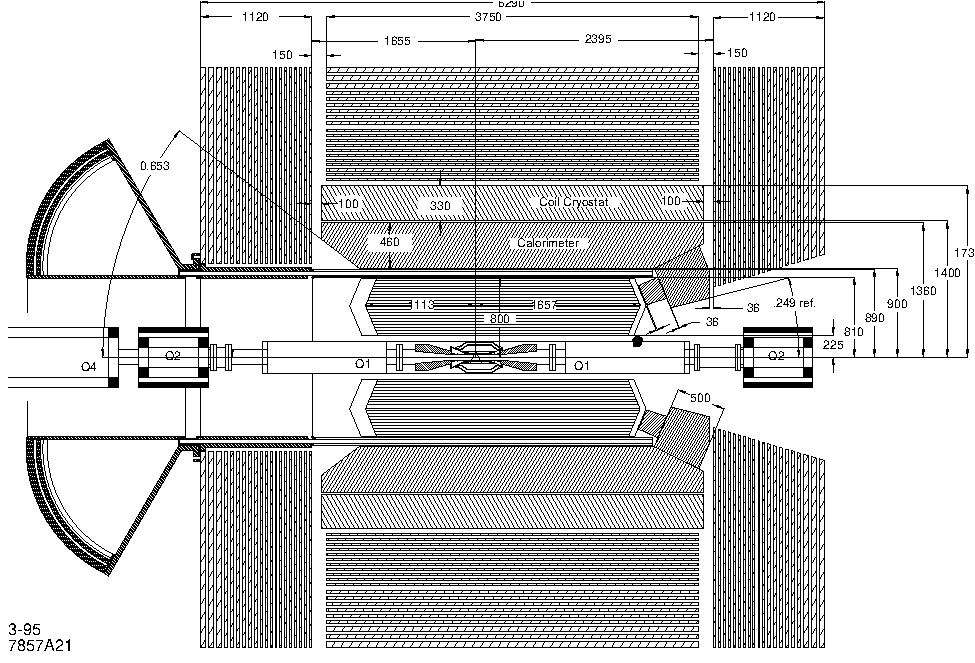
\includegraphics[width=0.7\textwidth]{figs/babar_detector_view.pdf}
    \caption{
        View of the \BaBar/ detector.
        Extracted from \cite{Boutigny:1995ib}.
    }
    \label{fig:babar_detector_view}
\end{figure}

% Talk about BaBar being 4 pi
In $e^- e^+$ detectors, $b \bar{b}$ is produced at all solid angles with
non-negligible probability \cite{Boutigny:1995ib,McGregor:2008ek}, thus the
detector needs to cover almost all solid angles (a $4\pi$ detector).
Indeed, \BaBar/ has tracking coverage of 0.92, namely 92\% of the $4\pi$ solid
angle.

% Talk about tracking and calorimeters
$B$ physics requires excellent vertex resolution and tracking, because the two
$B$ mesons produced by \Y4S/ must be reliably separated.
\BaBar/ has excellent tracking for charged particles, and sufficient spatial
and energy resolution in the electromagnetic calorimeter to reconstruct the
momenta of neutral particles \cite{Bauer:2005} with adequate precision.


\subsection{LHCb at the LHC} \label{sec:lhcb}
The LHC is a $pp$ collider, located at Geneva, Switzerland.
% Talk about the LHC being a hadron collider and the difficulties associated
% with it
Unlike electrons and positrons, the proton is a composite particle made of
$u, u, d$ quarks as well as other virtual partons.
All these particles participate in the $pp$ collision, carrying
varying portion of the total momentum.
The exact fraction of momentum carried by each type of parton is described by
parton distribution function\footnote{
    The parton distribution function is defined as:
    Number density to find fraction of the momentum (denoted as $x$) at certain
    squared energy scale $Q^2$.
} \cite{Ball:2014uwa}.
Since the precise fraction of momentum carried by interacting
partons\footnote{
    Again, these are characterized by parton distribution functions
} is unknown, the $B$ meson rest frame is not readily calculable.

Because many partons, such as quarks and gluons, can interact both
electroweakly and strongly,
the cross section of $b \bar{b}$ is larger than that of the $B$ factories, as a
result, more $b \bar{b}$ events are generated.
The measured $b \bar{b}$ cross section at LHCb in \SI{13}{TeV} $pp$
collisions\footnote{
    For $2 < \eta < 5$ only, since this is the LHCb acceptance range.
} is $144 \pm 1 \pm 21$~\si{\mu b} \cite{Aaij:2016avz}, whereas at the $B$
factories it is only about $1.05$~\si{nb} \cite{Harrison:1998yr}.
At the same time, unwanted particles will be generated frequently at hadron
colliders, leading to higher background.


% Talk about subdetectors
LHCb, a single-arm spectrometer, is one of the four large experiments at the
LHC.
Its constituent subdetectors, from closest to farthest from the collision point,
are shown in \autoref{fig:lhcb_detector_view}:
The Vertex Locator (VELO) provides precise measurements of track coordinates
close to the collision point.
Two Ring Imaging Cerencov counters (RICH1, RICH2) provide particle
identification for charged particles over a wide range of momentum.
The Tracker Turicensis (TT), Inner Tracker (IT), and Outer Tracker (OT) provide
additional tracking for charged particles and measure their momenta.
The calorimeters (ECAL and HCAL) have a first-level (L0) trigger to select
hadron, electron, and photon candidates based on their transverse momentum
$p_T$;
they also provide identification for the particles listed above;
finally, they provide energy and position measurements for these particles.
The Muon system (M1-5) is farthest from the collision point;
it provides L0 high $p_T$ muon trigger, and a high-level trigger (HLT) for muon
identification. Compared to the $B$ factories, LHCb has a much lower trigger
efficiency, which means many interesting events are filtered
out \cite{LHCb:2008}.

\begin{figure}[ht]
    \centering
    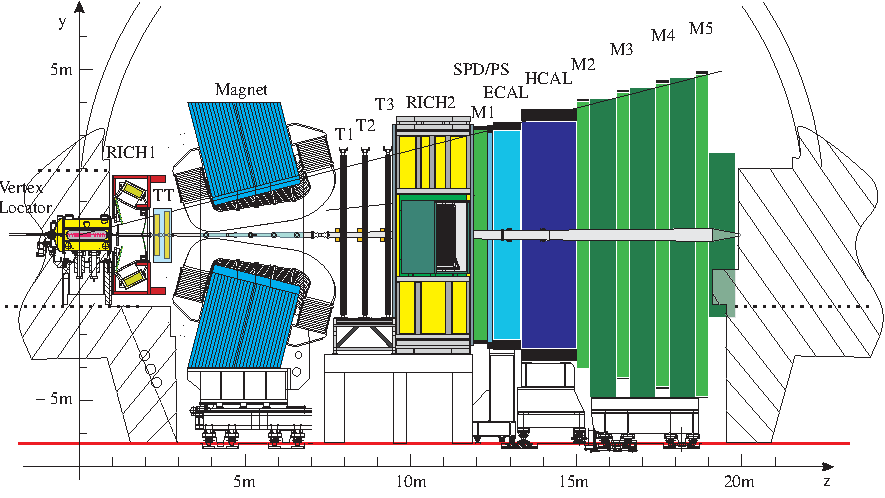
\includegraphics[width=0.7\textwidth]{figs/lhcb_detector_view.pdf}
    \caption{
        View of the LHCb detector and its subsystems.
        Extracted from \cite{LHCb:2003ab}.
    }
    \label{fig:lhcb_detector_view}
\end{figure}

% Talk about LHCb being forward-only
An interesting design choice is the geometry of the LHCb detector:
Instead of being a barrel $4\pi$ detector, it is forward-only.
This is because at high energies, $b\bar{b}$ is mostly produced in the forward
and backward direction.
The LHCb design is a very cost-effective way to construct a detector at the LHC
dedicated for $B$ physics.

% Talk about tracking
LHCb has a very good vertexing and tracking system, achieving vertex resolutions
down to 20~$\mu$m in a challenging environment.
However, due to the amount of material before the calorimeters and their poor
granularity,
reconstruction of neutral particles, such as $\pi_0$, is less
precise \cite{LHCb:2008,Guz:2017}.
This is why LHCb analyses typically focus on final states with charged particles
only, whereas $B$ factories can afford to use final states with neutral
particles.

% Talk about run 1 and run 2 luminosity
LHCb collected data from 2010 to 2012 with a center of mass energy of
\SI{8}{TeV}, and from 2015 to 2018 at \SI{13}{TeV}.
The total integrated luminosity during these two periods is about
\SI{9.2}{fb^{-1}} \cite{LHCb-Lumi:2019}.
% Talk about LS2 upgrade and LHCb's future
Currently, LHCb is shut down for an upgrade which will greatly increase the
readout rate of the detector starting in 2021.


\section{Review of previous measurements of \RDDst/}
In 2013, \BaBar/ reported a $3.4\sigma$ discrepancy in \RDDst/ from the
theoretical predictions \cite{Lees:2013rw}.
Since then, follow up measurements on the same semileptonic channel have been
performed by \BaBar/, BELLE, and LHCb, reporting various degrees of
discrepancies.
Currently, the world average of the measured \RDDst/ has a deviation of
$3.08\sigma$ with respect to SM prediction \cite{HFLAV:2019}, as shown
in \autoref{fig:rdrds_spring2019}.

\begin{figure}[ht]
    \centering
    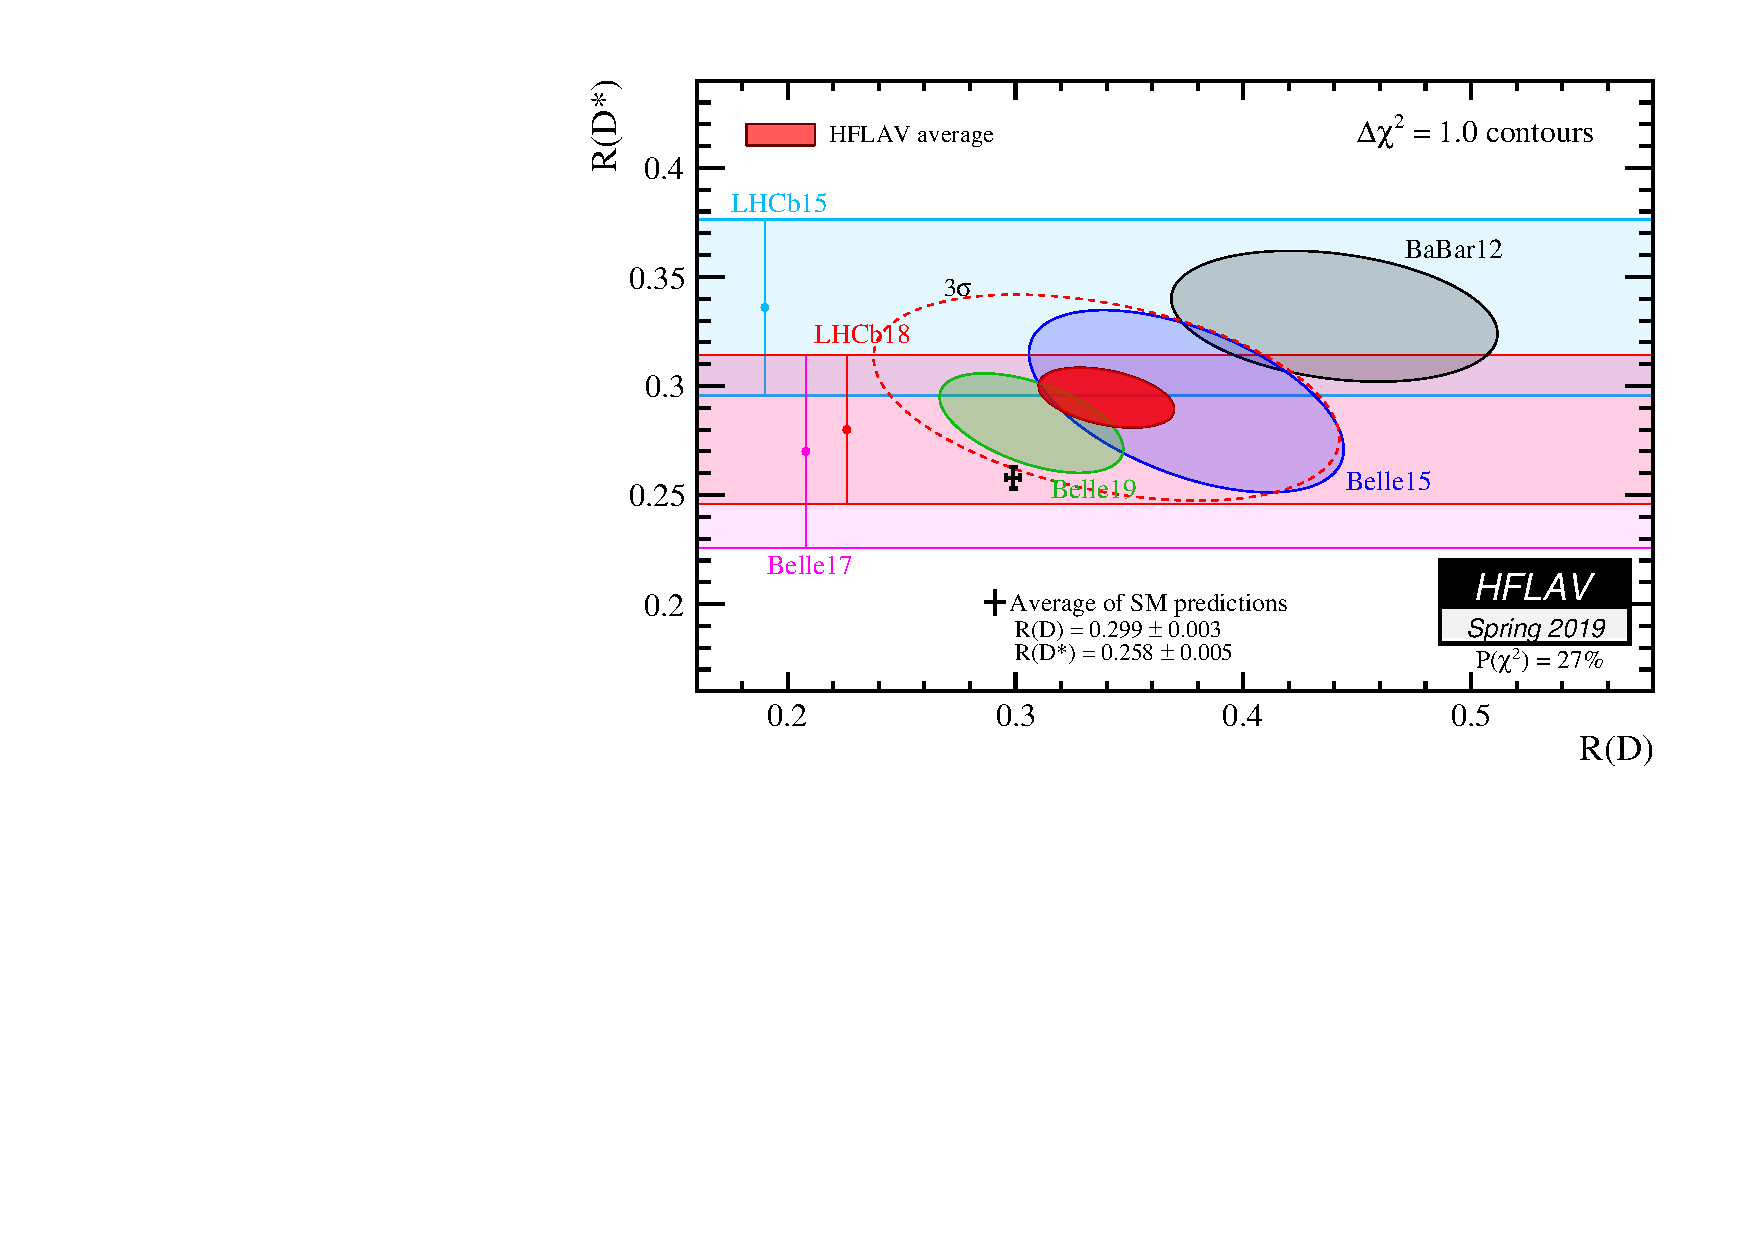
\includegraphics[width=0.6\textwidth]{figs/rdrds_spring2019.pdf}
    \caption{
        World average of measured \RD/ and \RDst/, and SM predictions, as of
        spring 2019.
    }
    \label{fig:rdrds_spring2019}
\end{figure}

% B-factory measurements
As mentioned in \autoref{sec:babar}, $B$ factories, such as \BaBar/ and BELLE,
know the momenta of the $B \overline{B}$ system exactly.
By tagging and reconstructing the other $B$, known as $B_{tag}$, the momentum of
the signal $B_{sig}$, which decays semileptonically, can be inferred.

\BaBar/ and BELLE independently developed two types of tagging algorithms:
semileptonic tagging and hadronic tagging.
Semileptonic tagging finds $B_{tag}$ with the following decay:
$B^- \rightarrow l^- \bar{\nu}_l$, where $l$ is a $e$ or $\mu$.
This has the advantage of a larger branching ratio, thus more ($\approx 1\%$)
\Y4S/ events are tagged.
However, in this type of events, at least two neutrinos are presents, which
makes the reconstruction of $p_{B_{sig}}$ less precise \cite{Ciezarek:2017yzh}.

On the other hand, hadronic tagging searches over a very large number of
hadronic decay chains of $B$ for each \Y4S/ event, tagging the ones that match
one of the known modes.
This has a smaller tagging rate ($\approx 0.3$), but because $B_{tag}$ decays
hadronically, no neutrino is present in the final product.
This makes the reconstructed momentum of $B_{sig}$ very
precise \cite{Lees:2013uzd,Ciezarek:2017yzh}.

$B$ factory analyses also choose a particular decay mode of $\tau$:
$\tau^- \rightarrow l^- \nu_\tau \bar{\nu}_l$.
Thus the signal mode will have three neutrinos in the final product,
whereas the normalization mode only one.
By looking at the missing mass of the $B_{sig}$, defined as:
\begin{equation}
    m^2_{miss} \equiv \left(p_{B_{sig}} - p_{visible}\right)^2
\end{equation}
The signal, which has a non-zero $m^2_{miss}$, can be readily differentiated
from the normalization, which does have a $m^2_{miss} \approx 0$.

Non-$B \overline{B}$ background and misreconstructed events are suppressed by
requiring a tag, together with the requirement of having a $D^{(*)}$ meson and a
charged lepton on $B_{sig}$ \cite{Ciezarek:2017yzh}.

The main background remaining is semileptonic $B$ decays to $D^{**}$, which has
similar $m^2_{miss}$ distribution to the signal.
They can be differentiated from the signal by looking at the distribution of
$E^{*}_l$, the energy of the charged lepton in the $B$ rest
frame, because the background distribution extends to higher
energy \cite{Ciezarek:2017yzh}.

The 2013 \BaBar/ result used a Gaussian non-parametric kernel estimator in the
fitting process, because it allows for straightforward treading between variance
and bias \cite{Lees:2013uzd}, resulting in a better fit result.

% BELLE measurements
Other than the \BaBar/ result mentioned at the beginning of this section,
BELLE measured semileptonic $B$ decays with $\tau$ decays both
leptonically and hadronically.
Both semileptonic and hadronic tagging were used for the leptonic $\tau$ decay;
for hadronic $\tau$ decay, only hadronic tag was used.
The overall \RDDst/ deviation from the SM is about
$2\sigma$ \cite{Hirose:2017185}.

However, $B$ factories are limited by their data sample size, as discussed
in \autoref{sec:lhcb}.
This is the main advantage of LHCb.

% 2015 LHCb leptonic tau decay
The 2015 LHCb \RDst/ result, the first \RDst/ measurement at a hadron collider,
is $2.1\sigma$ larger than SM prediction \cite{LHCb:PhysRevLett.115.111803}.
This analysis is heavily inspired by the preview $B$ factory measurements, with
a few caveats:
The $B \overline{B}$ rest frame is not known in a hadron collider;
a significant contribution to the background due to the following decay mode:
$B \rightarrow D^* H_c X$, as these decay modes have similar $m^2_{miss}$ and
$E^{*}_l$ distributions very similar to the signal \cite{Ciezarek:2017yzh};
because the charge neutral particle resolution is not very good, a particular
decay mode, namely $\overline{B}^0 \rightarrow D^{*+} \tau^- \bar{\nu}_\tau$, is
chosen so that all visible final state particles are charged.

Without the $B \overline{B}$ rest frame, tagging algorithms used in the $B$
factory measurements cannot be applied.
This problem is solved by \emph{rest frame approximation}, a technique developed
by the analysis:
Assuming $\vec{(p_{B})_T}$ is unchanged, approximate $(p_{B})_z$ by the
following:
\begin{equation}
    (p_{B})_z = \frac{m_B}{m_{reco}} (p_{reco})_z
\end{equation}
with $m_B$ the known $B$ mass.
This is shown to have sufficient resolution \cite{LHCb:PhysRevLett.115.111803}.

The additional hadronic background is constrained by templates generated by
simulated data sample, with additional correction fitted from the
$D^{*+} \mu^- K^{\pm}$ control sample \cite{LHCb:PhysRevLett.115.111803}.
From \autoref{fig:babar_lhcb_fit_comparison}, we see that backgrounds of $B$
factories and LHCb have very different composition.

\begin{figure}[ht]
    \centering
    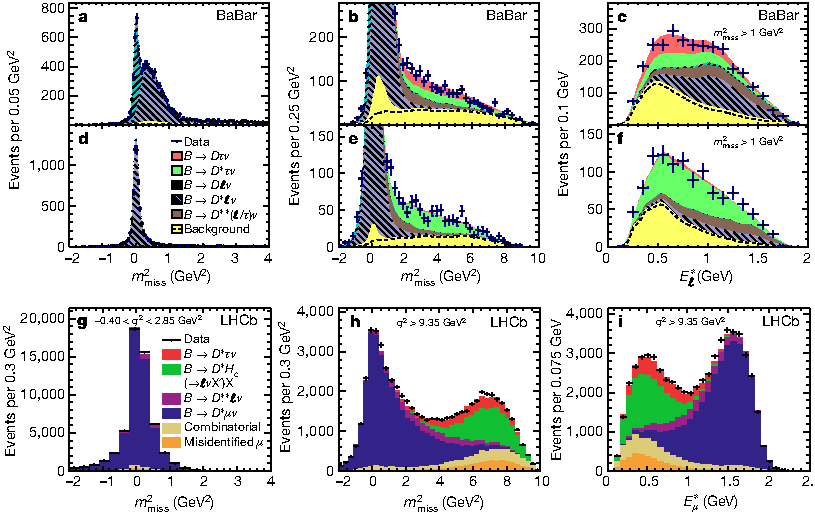
\includegraphics[width=0.85\textwidth]{figs/babar_lhcb_fit_comparison.pdf}
    \caption{
        Comparison between fitted data from \BaBar/ and LHCb.
    }
    \label{fig:babar_lhcb_fit_comparison}
\end{figure}

% 2018 LHCb hadronic tau decay: tau -> pi pi pi
The 2018 LHCb \RDst/ result is in agreement with the SM \cite{Aaij:2017deq}.
It used a different definition of \RDst/, renaming to $\mathcal{K}(D^{*-}))$:
\begin{equation}
    \mathcal{K}(D^{*-})) \equiv \frac{
        \mathcal{B}(B^0 \rightarrow D^{*-} \tau^+ \nu_\tau)
    }{
        \mathcal{B}(B^0 \rightarrow D^{*-} 3 \pi)
    }
\end{equation}

It also took a different approach to separate signal from normalization:
By using a different $t$ decay mode $\tau^- \rightarrow \pi^+ \pi^- \pi^+$,
the $\tau$ decay vertex can be reconstructed from the three charged pions.
Since $\tau$ flies a certain distance before it decays, its decay vertex is
separated from its generation vertex.
Thus, the signal events have a different topology than the normalization, of
which all final state particles point to the same vertex \cite{Aaij:2017deq}.

By requiring a clear separation between the two vertices, the prompt background
($D^* \pi \pi \pi X$) can be rejected.
The remaining double-charm background has the same topology as the signal.
A template derived from simulations is used to reject such
background \cite{Aaij:2017deq}.

\section{Outlook for LHCb Run 2 \RDDst/ measurements}
% Expected improvements
% Remember: Run 2 supposedly has better pile-ups.
% Current progress

\PRLrule
\printbibliography
\end{document}
